\chapter{Máy trạng thái}

Máy trạng thái là một trong những những kĩ thuật lập trình mình gặp nhiều nhất khi lập trình nhúng, dường như nó xuất hiện ở khắp nơi. Nắm vững kĩ thuật này thì code các bạn viết sẽ trở nên mạch lạc, sáng sủa hơn, và việc đọc code của người khác trở nên đơn giản hơn.
\newpage

\section{Blocking vs. Non-blocking}

Blocking là gì? Hãy xem qua chương trình chớp tắt led trong Arduino như sau:
\begin{lstlisting}
void loop() {
  digitalWrite(LED_BUILTIN, HIGH);   
  delay(1000);                       
  digitalWrite(LED_BUILTIN, LOW);    
  delay(1000);                       
}
\end{lstlisting}

Có thể thấy là nó bật led, sử dụng hàm \it{delay()} trong 1 giây rồi tắt led, tiếp tục \it{delay()} và chương trình lặp lại liên tục.

Vấn đề là ở chỗ hàm \it{delay()}, chương trình đứng yên một chỗ và không làm gì cả, hay nói cách khác là nó bị \it{block} tại chỗ đó. Viết chương trình có chứa hàm tạm dừng một chỗ như \it{delay()} thì người ta gọi là \textbf{Blocking mode}. Trong thế giới nhúng, tài nguyên hạn chế nên chương trình đứng một chỗ như vậy là việc hết sức lãng phí. 

Để khắc phục nhược điểm trên, người ta tạo ra kiểu có kiểu viết khác gọi là \textbf{Non-Blocking mode} nhằm làm cho chương trình chạy liên tục mà không bị kẹt tại một điểm nào cả. Kiểu viết này dựa trên máy trạng thái đơn giản như sau:

\begin{figure}[h!]
	\centering
\begin{tikzpicture}[->,>=stealth',shorten >=1pt,auto,node distance=5cm,
                    semithick]

  \node[initial,state] (A)                    	{$OFF$};
  \node[state]         (B) [right of=A] 		{$ON$};

  \path (A) edge [bend left]            node {1000ms} (B)
        (B) edge [bend left]            node {1000ms} (A);
 
\end{tikzpicture}
\caption{Máy trạng thái chớp tắt LED}
\end{figure}

Máy trạng thái như bạn thấy ở hình 2.1 là một biểu đồ các trạng thái của LED, hoặc của một đối tượng nào khác, và các điều kiện để chuyển từ trạng thái này sang trạng thái khác. Ở đây các trạng thái của LED bao gồm ON và OFF, điều kiện để chuyển đổi là sau mỗi 1 giây (1000 mili giây).

Sau khi vẽ ra sơ đồ, ta bắt đầu viết chương trình dựa trên lưu đồ trên như sau:

\begin{lstlisting}
void loop() {
    static uint32_t tick=0;
    static uint8_t led_state=LOW;
    if(millis()-tick>1000)
    {
        tick=millis();
        if(LOW==led_state){
            led_state=HIGH;
            digitalWrite(LED_BUILTIN, led_state);
        }
        else{
            led_state=LOW;
            digitalWrite(LED_BUILTIN, led_state);
        }
    }

    // Other code here
}
\end{lstlisting}

Biến \textit{tick} để lưu lại thời điểm của mỗi lần chuyển đổi trạng thái, biến \textit{state} để lưu lại trạng thái của LED. Do nằm trong hàm \textit{loop} nên hai biến này phải có khai báo \textit{static}.

Vòng \textit{loop} chạy lặp lại liên tục, mỗi lần chạy nó sẽ kiểm tra xem đã đủ 1000 mili giây chưa, sau đó tùy vào hiện trạng của LED hiện tại mà bật hay tắt LED, nó cũng cập nhật lại trạng thái mới và thời điểm chuyển đổi trạng thái.

Đây là ứng dụng đầu tiên của máy trạng thái, giúp các bạn có thể viết được dưới dạng \textbf{Non-blocking}, tiết kiệm tài nguyên CPU, có thể đa nhiệm hóa. Như ở dòng chú thích \textit{// Other code here}, bạn hoàn toàn có thể viết một chức năng khác, như điều khiển một LED khác, mà không lo bị ảnh hưởng bởi chương trình đã viết từ trước, với điều kiện là code mới của bạn cũng phải được viết ở dạng \textbf{Non-blocking}.

\section{Máy trạng thái cho chức năng của chương trình}

\textbf{Non-blocking} là một trong những ứng dụng của máy trạng thái để chương trình được chạy thông suốt và đa nhiệm tốt hơn. Nó giúp các chức năng chạy gần như song song và ít có ảnh hưởng tới nhau.

Tuy nhiên sức mạnh thực sự của máy trạng thái là ở khả năng bao quát được tính năng của chương trình. Nếu một máy trạng thái được viết tốt thì nó sẽ cho thấy cấu trúc của một chương trình, cách các tính năng phối hợp với nhau như thế nào để tạo ra một sản phẩm hoàn chỉnh, cách chương trình xử lí khi gặp lỗi...

Đặt vấn đề cho bài toán bơm nước vào bể như sau:

\begin{figure}[h!]
    \centering
     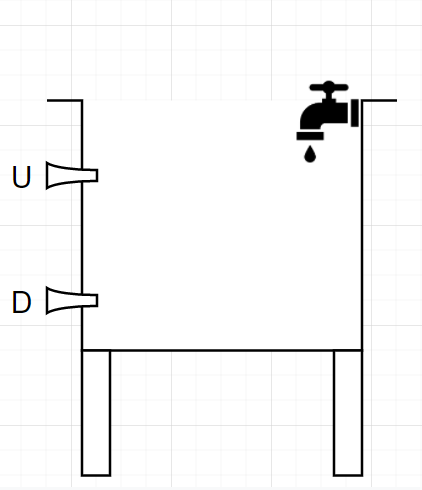
\includegraphics[width=0.6\linewidth]{images/tank.png}
     \caption{Bơm nước vào bể}
\end{figure}

Có một chiếc bể nước, có 1 vòi nước và 2 cảm biến mực nước trên (U) và dưới (D). Khi mực nước xuống thấp hơn cảm biến dưới (D=0), vòi nước được mở, nước bắt đầu được bơm vào. Khi mực nước vượt quá cảm biến trên (U=1) thì ngừng bơm.

Máy trạng thái của máy bơm sẽ như sau:

\begin{figure}[h!]
	\centering
\begin{tikzpicture}[->,>=stealth',shorten >=1pt,auto,node distance=5cm,
                    semithick]

  \node[initial,state] (A)                    	{$OFF$};
  \node[state]         (B) [right of=A] 		{$ON$};

  \path (A) edge [bend left]            node {D=0} (B)
        (B) edge [bend left]            node {U=1} (A);
 
\end{tikzpicture}
\caption{Máy bơm nước}
\end{figure}

\textbf{Bài tập}: các bạn dùng Ardino để làm bài tập này. Sử dụng 2 nút nhấn thay cho 2 cảm biến và đèn Led thay cho mô-tơ.

Và nếu chỉ đơn giản như vậy thì sẽ không phải là một sản phẩm có thể ứng dụng được thực tế. Trong thực tế sẽ có các trường hợp sau:

\begin{itemize}
    \item Bơm không lên nước do không có nước: khiến máy bơm chạy không tải liên tục, gây tốn điện và nhanh hư bơm.
    \item Bơm hoặc thiết bị đóng cắt hư.
    \item Cảm biến trên hư (U luôn bằng 0): Nước sẽ tràn ra ngoài, bơm không bao giờ dừng.
    \item Cảm biến trên hư (U luôn bằng 1): Nước sẽ dao động quanh cảm biến D, mô-tơ được bật tắt liên tục, nhanh hư mô-tơ và thiết bị đóng cắt mô-tơ.
    \item Cảm biến dưới hư (D luôn bằng 0): Giống như trường hợp trên, mực nước dao động quanh cảm biến U.
    \item Cảm biến dưới hư (D luôn bằng 1): Hết nước mà mô-tơ không bật.  
\end{itemize}

Một chương trình được viết tốt sẽ phát hiện được các lỗi có thể xảy ra trong thực tế, có biện pháp báo lỗi cho người dùng khi có sự cố, như nháy LED hoặc phát loa báo lỗi.

\textbf{Bài tập}: Hãy viết chương trình có tính năng báo lỗi khi hết nước hoặc bơm hư, hai cảm biến hoạt động bình thường. Khi phát hiện lỗi nháy một LED khác liên tục để báo lỗi.

Khi bơm vừa mới mới được bật, U=0, D=0, theo kinh nghiệm của mình thì rất nhanh sau đó D sẽ bằng 1, do mực nước đang tiệm cận D. Có thể xem giá trị này tối đa khoảng 1 phút, ta vẽ lại máy trạng thái như sau:

\begin{figure}[h!]
	\centering
\begin{tikzpicture}[->,>=stealth',shorten >=1pt,auto,node distance=5cm,
                    semithick]

  \node[initial,state] (A)                    	{$OFF$};
  \node[state]         (B) [right of=A] 		{$ON$};
  \node[state]         (C) [below of=B] 		{$Err$};

  \path (A) edge [bend left]            node {D=0} (B)
        (B) edge [bend left]            node {U=1} (A)
        (B) edge             node {D=0, t=60s} (C);
 
\end{tikzpicture}
\caption{Xử lí lỗi máy bơm}
\end{figure}

Khi rơi vào trạng thái lỗi, chương trình sẽ tắt máy bơm và nháy LED lỗi liên tục.

Đến một lỗi khác, khi đang bơm giữa chừng thì hết nước (lúc này D đã bằng 1). Nếu như theo lưu đồ trên thì bơm sẽ không bao giờ dừng. 

\textbf{Bài tập}: hãy viết chương trình để xử lí lỗi trên rồi quay lại đọc tiếp.

Để giải quyết vấn ta sẽ đặt ra một khoảng thời gian tối đa để bật bơm, dù cho cảm biến U có nhảy hay không. Giả sử ở đây mình sẽ cho thời gian tối đa là 600s (Hình 2.5).

\begin{figure}[h!]
	\centering
\begin{tikzpicture}[->,>=stealth',shorten >=1pt,auto,node distance=5cm,
                    semithick]

  \node[initial,state] (A)                    	{$OFF$};
  \node[state]         (B) [right of=A] 		{$ON$};
  \node[state]         (C) [below of=B] 		{$Err$};

  \path (A) edge [bend left]            node {D=0} (B)
        (B) edge [bend left]            node {U=1} (A)
        (B) edge [bend left]            node [below, rotate=90] {D=0, t>60s} (C)
        (B) edge [bend right]            node[above,rotate=90] {U=0, t>600s} (C);
 
\end{tikzpicture}
\caption{Xử lí lỗi máy bơm}
\end{figure}

Chúng ta có thể viết một lưu đồ khác với chức năng tương tự nhưng rõ ràng hơn (Hình 2.6).

\begin{figure}[h!]
	\centering
\begin{tikzpicture}[->,>=stealth',shorten >=1pt,auto,node distance=5cm,
                    semithick]

  \node[initial,state] (A)                    	{$OFF$};
  \node[state]         (B) [right of=A] 		{$Wait D$};
  \node[state]         (C) [below of=B] 		{$Err$};
  \node[state]         (D) [below of=A]        {$Wait U$};

  \path (A) edge             node {D=0} (B)
        (B) edge             node {D=1} (D)
        (B) edge             node {D=0, t>60s} (C)
        (D) edge           node {U=0, t>600s} (C)
        (D) edge                        node {U=1} (A)
        ;
 
\end{tikzpicture}
\caption{Xử lí lỗi máy bơm}
\end{figure}

\textit{Wait D} là trạng thái sau khi bật máy bơm, chương trình chờ cho đến khi cảm biến D nhảy. Sau đó chuyển sang \textit{Wait U}. Nếu trong quá trình chờ mà phát sinh lỗi thì sẽ chuyển sang báo lỗi. 

Còn các trường hợp lỗi cảm biến thì mong bạn đọc có thể tự vẽ lưu đồ và viết code để có thể xử lí hết các trường hợp lỗi có thể xảy ra.

Để làm cho một chương trình chạy đúng chức năng với các điều kiện lí tưởng thì không khó lắm. Tuy nhiên trong thực tế rất nhiều thứ xảy ra mà ta không thể lường trước được, nên việc phát triển sản phẩm là công việc liên tục từ lúc lên ý tưởng, hoàn thiện sản phẩm, đưa ra cho người dùng thử, lắng nghe những phản hồi và xử lí sự cố, cải tiến sản phẩm.

Đôi khi những trục trặc phát sinh trong quá trình chạy thực tế gây tổn thất rất nhiều thời gian và tiền bạc. Nếu có một vấn đề nào bạn có thể lường trước được khi còn trong phòng Lab thì nên giải quyết triệt để.

